\documentclass[11pt,compress,t,notes=noshow, xcolor=table]{beamer}
\documentclass[11pt,compress,t,notes=noshow, xcolor=table]{beamer}
\usepackage[]{graphicx}\usepackage[]{color}
% maxwidth is the original width if it is less than linewidth
% otherwise use linewidth (to make sure the graphics do not exceed the margin)
\makeatletter
\def\maxwidth{ %
  \ifdim\Gin@nat@width>\linewidth
    \linewidth
  \else
    \Gin@nat@width
  \fi
}
\makeatother

\definecolor{fgcolor}{rgb}{0.345, 0.345, 0.345}
\newcommand{\hlnum}[1]{\textcolor[rgb]{0.686,0.059,0.569}{#1}}%
\newcommand{\hlstr}[1]{\textcolor[rgb]{0.192,0.494,0.8}{#1}}%
\newcommand{\hlcom}[1]{\textcolor[rgb]{0.678,0.584,0.686}{\textit{#1}}}%
\newcommand{\hlopt}[1]{\textcolor[rgb]{0,0,0}{#1}}%
\newcommand{\hlstd}[1]{\textcolor[rgb]{0.345,0.345,0.345}{#1}}%
\newcommand{\hlkwa}[1]{\textcolor[rgb]{0.161,0.373,0.58}{\textbf{#1}}}%
\newcommand{\hlkwb}[1]{\textcolor[rgb]{0.69,0.353,0.396}{#1}}%
\newcommand{\hlkwc}[1]{\textcolor[rgb]{0.333,0.667,0.333}{#1}}%
\newcommand{\hlkwd}[1]{\textcolor[rgb]{0.737,0.353,0.396}{\textbf{#1}}}%
\let\hlipl\hlkwb

\usepackage{framed}
\makeatletter
\newenvironment{kframe}{%
 \def\at@end@of@kframe{}%
 \ifinner\ifhmode%
  \def\at@end@of@kframe{\end{minipage}}%
  \begin{minipage}{\columnwidth}%
 \fi\fi%
 \def\FrameCommand##1{\hskip\@totalleftmargin \hskip-\fboxsep
 \colorbox{shadecolor}{##1}\hskip-\fboxsep
     % There is no \\@totalrightmargin, so:
     \hskip-\linewidth \hskip-\@totalleftmargin \hskip\columnwidth}%
 \MakeFramed {\advance\hsize-\width
   \@totalleftmargin\z@ \linewidth\hsize
   \@setminipage}}%
 {\par\unskip\endMakeFramed%
 \at@end@of@kframe}
\makeatother

\definecolor{shadecolor}{rgb}{.97, .97, .97}
\definecolor{messagecolor}{rgb}{0, 0, 0}
\definecolor{warningcolor}{rgb}{1, 0, 1}
\definecolor{errorcolor}{rgb}{1, 0, 0}
\newenvironment{knitrout}{}{} % an empty environment to be redefined in TeX

\usepackage{alltt}
\newcommand{\SweaveOpts}[1]{}  % do not interfere with LaTeX
\newcommand{\SweaveInput}[1]{} % because they are not real TeX commands
\newcommand{\Sexpr}[1]{}       % will only be parsed by R
\newcommand{\xmark}{\ding{55}}%


\usepackage[english]{babel}
\usepackage[utf8]{inputenc}

\usepackage{dsfont}
\usepackage{verbatim}
\usepackage{amsmath}
\usepackage{amsfonts}
\usepackage{amssymb}
\usepackage{bm}
\usepackage{csquotes}
\usepackage{multirow}
\usepackage{longtable}
\usepackage{booktabs}
\usepackage{enumerate}
\usepackage[absolute,overlay]{textpos}
\usepackage{psfrag}
\usepackage{algorithm}
\usepackage{algpseudocode}
\usepackage{eqnarray}
\usepackage{arydshln}
\usepackage{tabularx}
\usepackage{placeins}
\usepackage{tikz}
\usepackage{setspace}
\usepackage{colortbl}
\usepackage{mathtools}
\usepackage{wrapfig}
\usepackage{bm}
\usepackage{amsmath}
\usepackage{pifont}

\usetikzlibrary{shapes,arrows,automata,positioning,calc,chains,trees, shadows}
\tikzset{
  %Define standard arrow tip
  >=stealth',
  %Define style for boxes
  punkt/.style={
    rectangle,
    rounded corners,
    draw=black, very thick,
    text width=6.5em,
    minimum height=2em,
    text centered},
  % Define arrow style
  pil/.style={
    ->,
    thick,
    shorten <=2pt,
    shorten >=2pt,}
}

\usepackage{subfig}

% Defines macros and environments
\usepackage{../../style/lmu-lecture}


\let\code=\texttt
\let\proglang=\textsf

\setkeys{Gin}{width=0.9\textwidth}

\setbeamertemplate{frametitle}{\expandafter\uppercase\expandafter\insertframetitle}

% This file is included in slides and exercises

% Rarely used fontstyle for R packages, used only in 
% - forests/slides-forests-benchmark.tex
% - exercises/single-exercises/methods_l_1.Rnw
% - slides/cart/attic/slides_extra_trees.Rnw
\newcommand{\pkg}[1]{{\fontseries{b}\selectfont #1}}

% Spacing helpers, used often (mostly in exercises for \dlz)
\newcommand{\lz}{\vspace{0.5cm}} % vertical space (used often in slides)
\newcommand{\dlz}{\vspace{1cm}}  % double vertical space (used often in exercises, never in slides)
\newcommand{\oneliner}[1] % Oneliner for important statements, used e.g. in iml, algods
{\begin{block}{}\begin{center}\begin{Large}#1\end{Large}\end{center}\end{block}}

% Don't know if this is used or needed, remove?
% textcolor that works in mathmode
% https://tex.stackexchange.com/a/261480
% Used e.g. in forests/slides-forests-bagging.tex
% [...] \textcolor{blue}{\tfrac{1}{M}\sum^M_{m} [...]
% \makeatletter
% \renewcommand*{\@textcolor}[3]{%
%   \protect\leavevmode
%   \begingroup
%     \color#1{#2}#3%
%   \endgroup
% }
% \makeatother






% latex-math includes as needed
% dependencies: amsmath, amssymb, dsfont
% math spaces
\ifdefined\N
\renewcommand{\N}{\mathds{N}} % N, naturals
\else \newcommand{\N}{\mathds{N}} \fi
\newcommand{\Z}{\mathds{Z}} % Z, integers
\newcommand{\Q}{\mathds{Q}} % Q, rationals
\newcommand{\R}{\mathds{R}} % R, reals
\ifdefined\C
\renewcommand{\C}{\mathds{C}} % C, complex
\else \newcommand{\C}{\mathds{C}} \fi
\newcommand{\continuous}{\mathcal{C}} % C, space of continuous functions
\newcommand{\M}{\mathcal{M}} % machine numbers
\newcommand{\epsm}{\epsilon_m} % maximum error

% counting / finite sets
\newcommand{\setzo}{\{0, 1\}} % set 0, 1
\newcommand{\setmp}{\{-1, +1\}} % set -1, 1
\newcommand{\unitint}{[0, 1]} % unit interval

% basic math stuff
\newcommand{\xt}{\tilde x} % x tilde
\newcommand{\argmin}{\mathop{\mathrm{arg\,min}}} % argmin
\newcommand{\argmax}{\mathop{\mathrm{arg\,max}}} % argmax
\newcommand{\argminlim}{\argmin\limits} % argmin with limits
\newcommand{\argmaxlim}{\argmax\limits} % argmax with limits
\newcommand{\sign}{\operatorname{sign}} % sign, signum
\newcommand{\I}{\mathbb{I}} % I, indicator
\newcommand{\order}{\mathcal{O}} % O, order
\newcommand{\bigO}{\mathcal{O}} % Big-O Landau
\newcommand{\littleo}{{o}} % Little-o Landau
\newcommand{\pd}[2]{\frac{\partial{#1}}{\partial #2}} % partial derivative
\newcommand{\floorlr}[1]{\left\lfloor #1 \right\rfloor} % floor
\newcommand{\ceillr}[1]{\left\lceil #1 \right\rceil} % ceiling
\newcommand{\indep}{\perp \!\!\! \perp} % independence symbol

% sums and products
\newcommand{\sumin}{\sum\limits_{i=1}^n} % summation from i=1 to n
\newcommand{\sumim}{\sum\limits_{i=1}^m} % summation from i=1 to m
\newcommand{\sumjn}{\sum\limits_{j=1}^n} % summation from j=1 to p
\newcommand{\sumjp}{\sum\limits_{j=1}^p} % summation from j=1 to p
\newcommand{\sumik}{\sum\limits_{i=1}^k} % summation from i=1 to k
\newcommand{\sumkg}{\sum\limits_{k=1}^g} % summation from k=1 to g
\newcommand{\sumjg}{\sum\limits_{j=1}^g} % summation from j=1 to g
\newcommand{\summM}{\sum\limits_{m=1}^M} % summation from m=1 to M
\newcommand{\meanin}{\frac{1}{n} \sum\limits_{i=1}^n} % mean from i=1 to n
\newcommand{\meanim}{\frac{1}{m} \sum\limits_{i=1}^m} % mean from i=1 to n
\newcommand{\meankg}{\frac{1}{g} \sum\limits_{k=1}^g} % mean from k=1 to g
\newcommand{\meanmM}{\frac{1}{M} \sum\limits_{m=1}^M} % mean from m=1 to M
\newcommand{\prodin}{\prod\limits_{i=1}^n} % product from i=1 to n
\newcommand{\prodkg}{\prod\limits_{k=1}^g} % product from k=1 to g
\newcommand{\prodjp}{\prod\limits_{j=1}^p} % product from j=1 to p

% linear algebra
\newcommand{\one}{\bm{1}} % 1, unitvector
\newcommand{\zero}{\mathbf{0}} % 0-vector
\newcommand{\id}{\bm{I}} % I, identity
\newcommand{\diag}{\operatorname{diag}} % diag, diagonal
\newcommand{\trace}{\operatorname{tr}} % tr, trace
\newcommand{\spn}{\operatorname{span}} % span
\newcommand{\scp}[2]{\left\langle #1, #2 \right\rangle} % <.,.>, scalarproduct
\newcommand{\mat}[1]{\begin{pmatrix} #1 \end{pmatrix}} % short pmatrix command
\newcommand{\Amat}{\mathbf{A}} % matrix A
\newcommand{\Deltab}{\mathbf{\Delta}} % error term for vectors

% basic probability + stats
\renewcommand{\P}{\mathds{P}} % P, probability
\newcommand{\E}{\mathds{E}} % E, expectation
\newcommand{\var}{\mathsf{Var}} % Var, variance
\newcommand{\cov}{\mathsf{Cov}} % Cov, covariance
\newcommand{\corr}{\mathsf{Corr}} % Corr, correlation
\newcommand{\normal}{\mathcal{N}} % N of the normal distribution
\newcommand{\iid}{\overset{i.i.d}{\sim}} % dist with i.i.d superscript
\newcommand{\distas}[1]{\overset{#1}{\sim}} % ... is distributed as ...

% machine learning
\newcommand{\Xspace}{\mathcal{X}} % X, input space
\newcommand{\Yspace}{\mathcal{Y}} % Y, output space
\newcommand{\Zspace}{\mathcal{Z}} % Z, space of sampled datapoints
\newcommand{\nset}{\{1, \ldots, n\}} % set from 1 to n
\newcommand{\pset}{\{1, \ldots, p\}} % set from 1 to p
\newcommand{\gset}{\{1, \ldots, g\}} % set from 1 to g
\newcommand{\Pxy}{\mathbb{P}_{xy}} % P_xy
\newcommand{\Exy}{\mathbb{E}_{xy}} % E_xy: Expectation over random variables xy
\newcommand{\xv}{\mathbf{x}} % vector x (bold)
\newcommand{\xtil}{\tilde{\mathbf{x}}} % vector x-tilde (bold)
\newcommand{\yv}{\mathbf{y}} % vector y (bold)
\newcommand{\xy}{(\xv, y)} % observation (x, y)
\newcommand{\xvec}{\left(x_1, \ldots, x_p\right)^\top} % (x1, ..., xp)
\newcommand{\Xmat}{\mathbf{X}} % Design matrix
\newcommand{\allDatasets}{\mathds{D}} % The set of all datasets
\newcommand{\allDatasetsn}{\mathds{D}_n}  % The set of all datasets of size n
\newcommand{\D}{\mathcal{D}} % D, data
\newcommand{\Dn}{\D_n} % D_n, data of size n
\newcommand{\Dtrain}{\mathcal{D}_{\text{train}}} % D_train, training set
\newcommand{\Dtest}{\mathcal{D}_{\text{test}}} % D_test, test set
\newcommand{\xyi}[1][i]{\left(\xv^{(#1)}, y^{(#1)}\right)} % (x^i, y^i), i-th observation
\newcommand{\Dset}{\left( \xyi[1], \ldots, \xyi[n]\right)} % {(x1,y1)), ..., (xn,yn)}, data
\newcommand{\defAllDatasetsn}{(\Xspace \times \Yspace)^n} % Def. of the set of all datasets of size n
\newcommand{\defAllDatasets}{\bigcup_{n \in \N}(\Xspace \times \Yspace)^n} % Def. of the set of all datasets
\newcommand{\xdat}{\left\{ \xv^{(1)}, \ldots, \xv^{(n)}\right\}} % {x1, ..., xn}, input data
\newcommand{\ydat}{\left\{ \yv^{(1)}, \ldots, \yv^{(n)}\right\}} % {y1, ..., yn}, input data
\newcommand{\yvec}{\left(y^{(1)}, \hdots, y^{(n)}\right)^\top} % (y1, ..., yn), vector of outcomes
\newcommand{\greekxi}{\xi} % Greek letter xi
\renewcommand{\xi}[1][i]{\xv^{(#1)}} % x^i, i-th observed value of x
\newcommand{\yi}[1][i]{y^{(#1)}} % y^i, i-th observed value of y
\newcommand{\xivec}{\left(x^{(i)}_1, \ldots, x^{(i)}_p\right)^\top} % (x1^i, ..., xp^i), i-th observation vector
\newcommand{\xj}{\xv_j} % x_j, j-th feature
\newcommand{\xjvec}{\left(x^{(1)}_j, \ldots, x^{(n)}_j\right)^\top} % (x^1_j, ..., x^n_j), j-th feature vector
\newcommand{\phiv}{\mathbf{\phi}} % Basis transformation function phi
\newcommand{\phixi}{\mathbf{\phi}^{(i)}} % Basis transformation of xi: phi^i := phi(xi)

%%%%%% ml - models general
\newcommand{\lamv}{\bm{\lambda}} % lambda vector, hyperconfiguration vector
\newcommand{\Lam}{\bm{\Lambda}}	 % Lambda, space of all hpos
% Inducer / Inducing algorithm
\newcommand{\preimageInducer}{\left(\defAllDatasets\right)\times\Lam} % Set of all datasets times the hyperparameter space
\newcommand{\preimageInducerShort}{\allDatasets\times\Lam} % Set of all datasets times the hyperparameter space
% Inducer / Inducing algorithm
\newcommand{\ind}{\mathcal{I}} % Inducer, inducing algorithm, learning algorithm

% continuous prediction function f
\newcommand{\ftrue}{f_{\text{true}}}  % True underlying function (if a statistical model is assumed)
\newcommand{\ftruex}{\ftrue(\xv)} % True underlying function (if a statistical model is assumed)
\newcommand{\fx}{f(\xv)} % f(x), continuous prediction function
\newcommand{\fdomains}{f: \Xspace \rightarrow \R^g} % f with domain and co-domain
\newcommand{\Hspace}{\mathcal{H}} % hypothesis space where f is from
\newcommand{\fbayes}{f^{\ast}} % Bayes-optimal model
\newcommand{\fxbayes}{f^{\ast}(\xv)} % Bayes-optimal model
\newcommand{\fkx}[1][k]{f_{#1}(\xv)} % f_j(x), discriminant component function
\newcommand{\fh}{\hat{f}} % f hat, estimated prediction function
\newcommand{\fxh}{\fh(\xv)} % fhat(x)
\newcommand{\fxt}{f(\xv ~|~ \thetav)} % f(x | theta)
\newcommand{\fxi}{f\left(\xv^{(i)}\right)} % f(x^(i))
\newcommand{\fxih}{\hat{f}\left(\xv^{(i)}\right)} % f(x^(i))
\newcommand{\fxit}{f\left(\xv^{(i)} ~|~ \thetav\right)} % f(x^(i) | theta)
\newcommand{\fhD}{\fh_{\D}} % fhat_D, estimate of f based on D
\newcommand{\fhDtrain}{\fh_{\Dtrain}} % fhat_Dtrain, estimate of f based on D
\newcommand{\fhDnlam}{\fh_{\Dn, \lamv}} %model learned on Dn with hp lambda
\newcommand{\fhDlam}{\fh_{\D, \lamv}} %model learned on D with hp lambda
\newcommand{\fhDnlams}{\fh_{\Dn, \lamv^\ast}} %model learned on Dn with optimal hp lambda
\newcommand{\fhDlams}{\fh_{\D, \lamv^\ast}} %model learned on D with optimal hp lambda

% discrete prediction function h
\newcommand{\hx}{h(\xv)} % h(x), discrete prediction function
\newcommand{\hh}{\hat{h}} % h hat
\newcommand{\hxh}{\hat{h}(\xv)} % hhat(x)
\newcommand{\hxt}{h(\xv | \thetav)} % h(x | theta)
\newcommand{\hxi}{h\left(\xi\right)} % h(x^(i))
\newcommand{\hxit}{h\left(\xi ~|~ \thetav\right)} % h(x^(i) | theta)
\newcommand{\hbayes}{h^{\ast}} % Bayes-optimal classification model
\newcommand{\hxbayes}{h^{\ast}(\xv)} % Bayes-optimal classification model

% yhat
\newcommand{\yh}{\hat{y}} % yhat for prediction of target
\newcommand{\yih}{\hat{y}^{(i)}} % yhat^(i) for prediction of ith targiet
\newcommand{\resi}{\yi- \yih}

% theta
\newcommand{\thetah}{\hat{\theta}} % theta hat
\newcommand{\thetav}{\bm{\theta}} % theta vector
\newcommand{\thetavh}{\bm{\hat\theta}} % theta vector hat
\newcommand{\thetat}[1][t]{\thetav^{[#1]}} % theta^[t] in optimization
\newcommand{\thetatn}[1][t]{\thetav^{[#1 +1]}} % theta^[t+1] in optimization
\newcommand{\thetahDnlam}{\thetavh_{\Dn, \lamv}} %theta learned on Dn with hp lambda
\newcommand{\thetahDlam}{\thetavh_{\D, \lamv}} %theta learned on D with hp lambda
\newcommand{\mint}{\min_{\thetav \in \Theta}} % min problem theta
\newcommand{\argmint}{\argmin_{\thetav \in \Theta}} % argmin theta

% densities + probabilities
% pdf of x
\newcommand{\pdf}{p} % p
\newcommand{\pdfx}{p(\xv)} % p(x)
\newcommand{\pixt}{\pi(\xv~|~ \thetav)} % pi(x|theta), pdf of x given theta
\newcommand{\pixit}[1][i]{\pi\left(\xi[#1] ~|~ \thetav\right)} % pi(x^i|theta), pdf of x given theta
\newcommand{\pixii}[1][i]{\pi\left(\xi[#1]\right)} % pi(x^i), pdf of i-th x

% pdf of (x, y)
\newcommand{\pdfxy}{p(\xv,y)} % p(x, y)
\newcommand{\pdfxyt}{p(\xv, y ~|~ \thetav)} % p(x, y | theta)
\newcommand{\pdfxyit}{p\left(\xi, \yi ~|~ \thetav\right)} % p(x^(i), y^(i) | theta)

% pdf of x given y
\newcommand{\pdfxyk}[1][k]{p(\xv | y= #1)} % p(x | y = k)
\newcommand{\lpdfxyk}[1][k]{\log p(\xv | y= #1)} % log p(x | y = k)
\newcommand{\pdfxiyk}[1][k]{p\left(\xi | y= #1 \right)} % p(x^i | y = k)

% prior probabilities
\newcommand{\pik}[1][k]{\pi_{#1}} % pi_k, prior
\newcommand{\lpik}[1][k]{\log \pi_{#1}} % log pi_k, log of the prior
\newcommand{\pit}{\pi(\thetav)} % Prior probability of parameter theta

% posterior probabilities
\newcommand{\post}{\P(y = 1 ~|~ \xv)} % P(y = 1 | x), post. prob for y=1
\newcommand{\postk}[1][k]{\P(y = #1 ~|~ \xv)} % P(y = k | y), post. prob for y=k
\newcommand{\pidomains}{\pi: \Xspace \rightarrow \unitint} % pi with domain and co-domain
\newcommand{\pibayes}{\pi^{\ast}} % Bayes-optimal classification model
\newcommand{\pixbayes}{\pi^{\ast}(\xv)} % Bayes-optimal classification model
\newcommand{\pix}{\pi(\xv)} % pi(x), P(y = 1 | x)
\newcommand{\piv}{\bm{\pi}} % pi, bold, as vector
\newcommand{\pikx}[1][k]{\pi_{#1}(\xv)} % pi_k(x), P(y = k | x)
\newcommand{\pikxt}[1][k]{\pi_{#1}(\xv ~|~ \thetav)} % pi_k(x | theta), P(y = k | x, theta)
\newcommand{\pixh}{\hat \pi(\xv)} % pi(x) hat, P(y = 1 | x) hat
\newcommand{\pikxh}[1][k]{\hat \pi_{#1}(\xv)} % pi_k(x) hat, P(y = k | x) hat
\newcommand{\pixih}{\hat \pi(\xi)} % pi(x^(i)) with hat
\newcommand{\pikxih}[1][k]{\hat \pi_{#1}(\xi)} % pi_k(x^(i)) with hat
\newcommand{\pdfygxt}{p(y ~|~\xv, \thetav)} % p(y | x, theta)
\newcommand{\pdfyigxit}{p\left(\yi ~|~\xi, \thetav\right)} % p(y^i |x^i, theta)
\newcommand{\lpdfygxt}{\log \pdfygxt } % log p(y | x, theta)
\newcommand{\lpdfyigxit}{\log \pdfyigxit} % log p(y^i |x^i, theta)

% probababilistic
\newcommand{\bayesrulek}[1][k]{\frac{\P(\xv | y= #1) \P(y= #1)}{\P(\xv)}} % Bayes rule
\newcommand{\muk}{\bm{\mu_k}} % mean vector of class-k Gaussian (discr analysis)

% residual and margin
\newcommand{\eps}{\epsilon} % residual, stochastic
\newcommand{\epsv}{\bm{\epsilon}} % residual, stochastic, as vector
\newcommand{\epsi}{\epsilon^{(i)}} % epsilon^i, residual, stochastic
\newcommand{\epsh}{\hat{\epsilon}} % residual, estimated
\newcommand{\epsvh}{\hat{\epsv}} % residual, estimated, vector
\newcommand{\yf}{y \fx} % y f(x), margin
\newcommand{\yfi}{\yi \fxi} % y^i f(x^i), margin
\newcommand{\Sigmah}{\hat \Sigma} % estimated covariance matrix
\newcommand{\Sigmahj}{\hat \Sigma_j} % estimated covariance matrix for the j-th class

% ml - loss, risk, likelihood
\newcommand{\Lyf}{L\left(y, f\right)} % L(y, f), loss function
\newcommand{\Lypi}{L\left(y, \pi\right)} % L(y, pi), loss function
\newcommand{\Lxy}{L\left(y, \fx\right)} % L(y, f(x)), loss function
\newcommand{\Lxyi}{L\left(\yi, \fxi\right)} % loss of observation
\newcommand{\Lxyt}{L\left(y, \fxt\right)} % loss with f parameterized
\newcommand{\Lxyit}{L\left(\yi, \fxit\right)} % loss of observation with f parameterized
\newcommand{\Lxym}{L\left(\yi, f\left(\bm{\tilde{x}}^{(i)} ~|~ \thetav\right)\right)} % loss of observation with f parameterized
\newcommand{\Lpixy}{L\left(y, \pix\right)} % loss in classification
\newcommand{\Lpiy}{L\left(y, \pi\right)} % loss in classification
\newcommand{\Lpiv}{L\left(y, \piv\right)} % loss in classification
\newcommand{\Lpixyi}{L\left(\yi, \pixii\right)} % loss of observation in classification
\newcommand{\Lpixyt}{L\left(y, \pixt\right)} % loss with pi parameterized
\newcommand{\Lpixyit}{L\left(\yi, \pixit\right)} % loss of observation with pi parameterized
\newcommand{\Lhy}{L\left(y, h\right)} % L(y, h), loss function on discrete classes
\newcommand{\Lhxy}{L\left(y, \hx\right)} % L(y, h(x)), loss function on discrete classes
\newcommand{\Lr}{L\left(r\right)} % L(r), loss defined on residual (reg) / margin (classif)
\newcommand{\lone}{|y - \fx|} % L1 loss
\newcommand{\ltwo}{\left(y - \fx\right)^2} % L2 loss
\newcommand{\lbernoullimp}{\ln(1 + \exp(-y \cdot \fx))} % Bernoulli loss for -1, +1 encoding
\newcommand{\lbernoullizo}{- y \cdot \fx + \log(1 + \exp(\fx))} % Bernoulli loss for 0, 1 encoding
\newcommand{\lcrossent}{- y \log \left(\pix\right) - (1 - y) \log \left(1 - \pix\right)} % cross-entropy loss
\newcommand{\lbrier}{\left(\pix - y \right)^2} % Brier score
\newcommand{\risk}{\mathcal{R}} % R, risk
\newcommand{\riskbayes}{\mathcal{R}^\ast}
\newcommand{\riskf}{\risk(f)} % R(f), risk
\newcommand{\riskdef}{\E_{y|\xv}\left(\Lxy \right)} % risk def (expected loss)
\newcommand{\riskt}{\mathcal{R}(\thetav)} % R(theta), risk
\newcommand{\riske}{\mathcal{R}_{\text{emp}}} % R_emp, empirical risk w/o factor 1 / n
\newcommand{\riskeb}{\bar{\mathcal{R}}_{\text{emp}}} % R_emp, empirical risk w/ factor 1 / n
\newcommand{\riskef}{\riske(f)} % R_emp(f)
\newcommand{\risket}{\mathcal{R}_{\text{emp}}(\thetav)} % R_emp(theta)
\newcommand{\riskr}{\mathcal{R}_{\text{reg}}} % R_reg, regularized risk
\newcommand{\riskrt}{\mathcal{R}_{\text{reg}}(\thetav)} % R_reg(theta)
\newcommand{\riskrf}{\riskr(f)} % R_reg(f)
\newcommand{\riskrth}{\hat{\mathcal{R}}_{\text{reg}}(\thetav)} % hat R_reg(theta)
\newcommand{\risketh}{\hat{\mathcal{R}}_{\text{emp}}(\thetav)} % hat R_emp(theta)
\newcommand{\LL}{\mathcal{L}} % L, likelihood
\newcommand{\LLt}{\mathcal{L}(\thetav)} % L(theta), likelihood
\newcommand{\LLtx}{\mathcal{L}(\thetav | \xv)} % L(theta|x), likelihood
\newcommand{\logl}{\ell} % l, log-likelihood
\newcommand{\loglt}{\logl(\thetav)} % l(theta), log-likelihood
\newcommand{\logltx}{\logl(\thetav | \xv)} % l(theta|x), log-likelihood
\newcommand{\errtrain}{\text{err}_{\text{train}}} % training error
\newcommand{\errtest}{\text{err}_{\text{test}}} % test error
\newcommand{\errexp}{\overline{\text{err}_{\text{test}}}} % avg training error

% lm
\newcommand{\thx}{\thetav^\top \xv} % linear model
\newcommand{\olsest}{(\Xmat^\top \Xmat)^{-1} \Xmat^\top \yv} % OLS estimator in LM


% Lecture title always has to be there
\title{Algorithms and Data Structures}

\begin{document}

\titlemeta{% Chunk title (example: CART, Forests, Boosting, ...), can be empty
Quadrature
}{% Lecture title
Monte Carlo Integration
}{% Relative path to title page image: Can be empty but must not start with slides/
}{% Learning goals, wrapped inside itemize environment
  \item Simple Monte Carlo
  \item Hit-or-Miss approach
}

%\lecture{CIM1 Statistical Computing}

\begin{vbframe}{Simple Monte Carlo}

\textbf{Goal:} Calculate $I(f) = \int_a^b f(x)~dx$

\begin{itemize}
\item We define
$$
I(f) = (b - a)\int_a^b f(x)\cdot \frac{1}{b - a}~dx = (b - a)\cdot \E[f(x)]
$$
with $x \sim U(a, b)$
\item With $x_i \overset{iid}{\sim} U(a, b), i = 1, ..., n$ the Monte Carlo estimation is given by

$$
Q_{MC}(f) = \frac{b - a}{n} \sumin f(x_i)
$$
\item By "sampling" $n$ independent random numbers from $U(a,b)$ an estimate for the integral can be calculated.
\end{itemize}

\framebreak

Monte Carlo is a \textbf{non-deterministic} approach. The estimation for the integral $\int_a^b f(x) ~dx$ is subject to randomness:

\begin{itemize}
\item The strong law of large numbers states that $Q_{MC}(f)$ converges almost certainly towards $I(f) = \E[f(x)]$ for $n\to\infty$
\item We can derive the variance from $Q_{MC}(f)$:
\vspace*{-0.2cm}
\begin{eqnarray*}
\text{Var}\left(Q_{MC}(f)\right) &=& \text{Var}\left(\frac{b - a}{n} \sumin f(x_i)\right) \\
&\overset{iid}{=}& \frac{(b - a)^2}{n^2}\cdot n \cdot \text{Var}(f(x)) = \frac{(b - a)^2}{n} \sigma^2
\end{eqnarray*}
where $\sigma^2 = \text{Var}(f(x))$ denotes the variance of the random variable $f(x)$ with $x \sim U(a, b)$ which can be empirically estimated by \begin{footnotesize}$\hat \sigma^2 = \frac{1}{n - 1} \sumin \left(f(x_i) - \frac{1}{n}\sumin f(x_i)\right)^2, x_i \overset{iid}{\sim} U(a, b)$\end{footnotesize}.

\framebreak

% \item Mit $\hat \sigma^2 = \sumin \frac{\left(f(x_i) - \frac{1}{n}\sumin f(x_i)\right)^2}{n - 1}$ kann Varianz von $Q_{MC}(f)$ geschätzt werden
% \begin{eqnarray*}
% \widehat{\text{Var}}\left(Q_{MC}(f)\right) &=& \frac{(b - a)^2}{n} \cdot \sumin \frac{\left(f(x_i) - \frac{1}{n}\sumin f(x_i)\right)^2}{n - 1}.
% \end{eqnarray*}

\item If $\sigma^2 < \infty$ the variance of the estimate (and thus also the worst case error of the procedure) approaches $0$ for $n \to \infty$
\item Monte Carlo also works well in multidimensional settings:
\vspace*{-0.2cm}
\begin{itemize}
\item The Monte Carlo integration can simply be generalized to multidimensional integrals $\int_\Omega f(\bm{x}) ~ d\bm{x}$ with $\Omega \subset \R^d$ by drawing the random variables uniformly distributed in the $d$-dimensional space $\Omega$.
\item The variance is then
$$
    \text{Var}\left(Q_{MC}(f)\right) = \frac{V^2}{n} \sigma^2, \quad V = \int_\Omega ~ d\bm{x}
$$
\item In particular, the speed of convergence for the variance \textbf{does not} depend on the dimension of the function to be integrated.
\end{itemize}
\end{itemize}
\end{vbframe}



\begin{vbframe}{Hit-or-Miss}

\textbf{Idea:}

We draw $n$ independently uniformly distributed data points from a rectangle enclosing our function:

\begin{center}
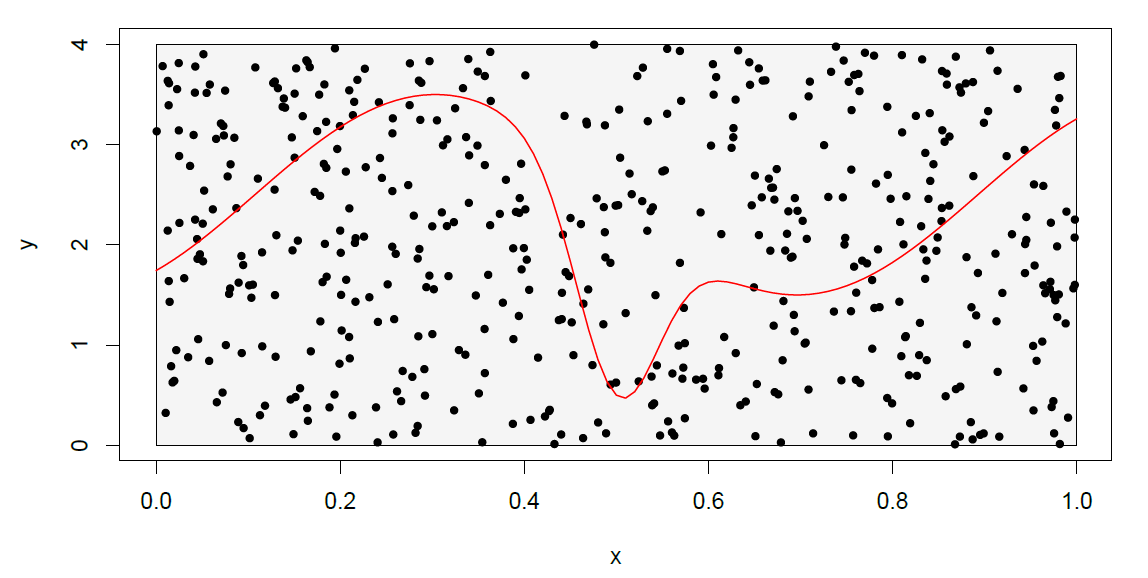
\includegraphics[width =0.7\textwidth]{figure_man/hitormiss.png}
\end{center}

\framebreak

\textbf{"Hit-or-Miss" Approach:}


We still consider the integral $\int_a^b f(x) dx$. We assume that $0 \le f(x) \le c$. If we count the number of hits (the points underneath the curve), we obtain the integral by:

$$
  I(f) \approx \frac{Hits}{n} \cdot \text{area of the rectangle} = \frac{\sumin \mathbf{1}_{y_i \le f(x_i)}}{n} \cdot c \cdot (b - a)
$$

\vspace*{-0.3cm}

\begin{center}
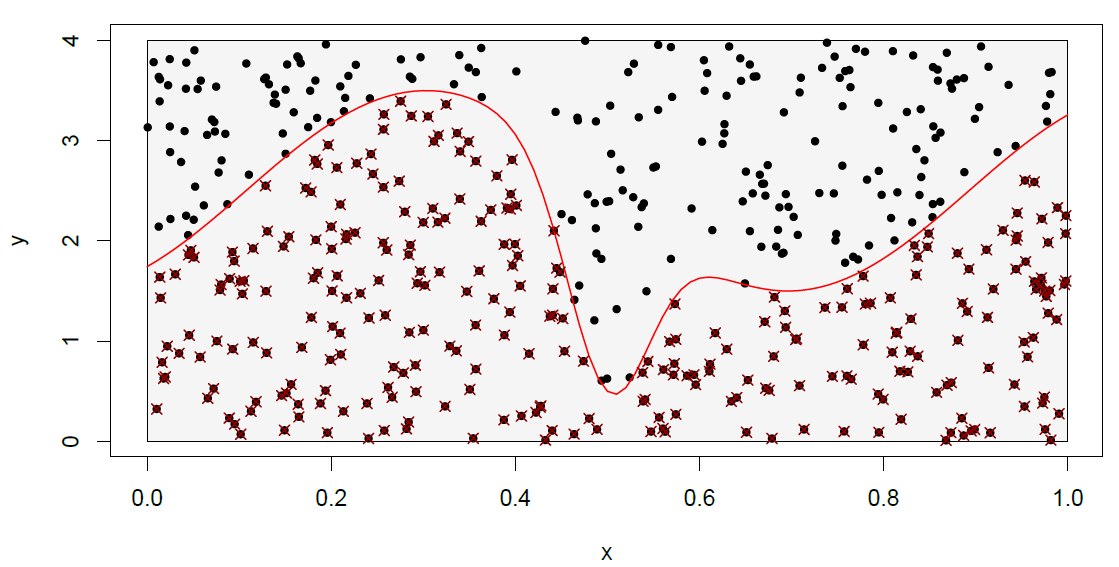
\includegraphics[width =0.68\textwidth]{figure_man/hitormiss2.png}
\end{center}


\framebreak


\footnotesize
\begin{verbatim}
m$estimate # Estimation of area
## [1] 2.288
m$hits # Number of points underneath the curve
## [1] 286
\end{verbatim}



\normalsize
$$
  I(f) \approx \frac{286}{500} \cdot \text{1 * 4} = 2.288
$$

This naive method works well for simple examples, but error rates are high for more complex applications.

\framebreak






% \framebreak
%
% \textbf{Anwendung:} Bayesian Computations
%
% \lz
%
% \textbf{Ziel:} Berechnung des Posterior-Erwartungswert $
% E(\theta | \xv) = \int \theta f(\theta | \xv)d\theta$
%
% \lz
%
% \begin{itemize}
% \item Angenommen, unabhängige Samples $\theta^{(1)}, \ldots, \theta^{(T)}$ aus
% $f(\theta | \xv)$ können einfach erzeugt werden.
% \item Eine Monte-Carlo-Schätzung des Posterior-Mittelwerts ist dann
% $$
% \hat{E}(\theta | \xv) = \frac{1}{T} \sum_{t = 1}^T \theta^{(t)}.
% $$
% \item Der Schätzer konvergiert zum wahren Posterior-Mittelwert konvergiert für $T \rightarrow \infty$ (Gesetz der großen Zahlen).
% \end{itemize}
% % Fehlerrate ist $\mathcal{O}(\frac{1}{\sqrt{T}})$. Relativ langsamer Algorithmus, aber sehr einfach,
% % falls Zufallszahlengenerator e\xvistiert.
% %
% \framebreak
%
%
% Die allgemeinere Form
%
% $$
% \hat{E}(g(\theta) | \xv) = \frac{1}{T} \sum_{t = 1}^T g(\theta^{(t)})
% $$
%
% ist ebenfalls konsistent.
%
% \lz
%
% Somit kann beispielsweise die Posterior-Varianz
% $$
% \widehat{Var}(\theta | \xv) = \hat{E}(\theta^2 | \xv) - \hat{E}(\theta | \xv)^2.
% $$
%
% \lz
%
% oder die kumulative Posterior-Verteilungsfunktion
%
% $$
% P(\theta \leq \theta_0) | \xv)
% $$
% mit Hilfe von Indikatorfunktionen $g(\theta) = I_{(-\infty, \theta_0]}(\theta)$ berechnet werden.
%
% \frembreak
%
%
% Wenn die Samples $\theta^{(t)}$ nicht wirklich unabhängig sind, betrifft das lediglich
% die Genauigkeit von $\hat{E}(g(\theta) | \xv)$.

\framebreak

\textbf{Advantages:}
\begin{itemize}
\item Monte Carlo integration does not require continuity for $f$
\item Error does not depend on the dimension (in contrast to deterministic quadrature formulas), but only on the variance of the function $f$ and the number of simulations $n$
\begin{itemize}
\item $\to$ Improve precision through high number of simulations
\item $\to$ Improve precision by reducing variance
\end{itemize}
\end{itemize}

\textbf{Disadvantages:}
\begin{itemize}
\item Relatively slow convergence rates
% \item setzt voraus, dass von $f(\theta|\xv)$ simuliert werden kann
\end{itemize}


% Trapezregel und Rechtecksregel haben Fehler der Ordnung $h^2$ (auch in höheren Dimensionen).
%
% \lz
%
% Das entspricht:
% \begin{itemize}
% \item Eindimensional:  $\mathcal{O}(\frac{1}{N^2})$.
% \item Zweidimensional: $\mathcal{O}(\frac{1}{N})$.
% \item Vierdimensional: $\mathcal{O}(\frac{1}{\sqrt N})$.
% \end{itemize}
% Dies ist der \textbf{Fluch der Dimensionalität}.

% \lz
%
% Vorteile der Monte-Carlo-Integration:
% \begin{itemize}
% \item Konvergenzrate unabhängig von Dimension. Ab Dimensionen 4 wird Monte-Carlo kompetitiv.
% \item Numerische Quadratur am besten, wenn $f$ glatt, z.B. Simpson $\mathcal{O}(h^4)$.
% \end{itemize}

\begin{center}
\begin{scriptsize}
\begin{verbatim}
set.seed(333)

T = 10000; shape = 2; rate = 1 / 2
theta = rgamma(T, shape = shape, rate = rate)

hist(theta, freq = FALSE, ylim = c(0, 0.2), main = "")
lines(density(theta))
\end{verbatim}
\end{scriptsize}

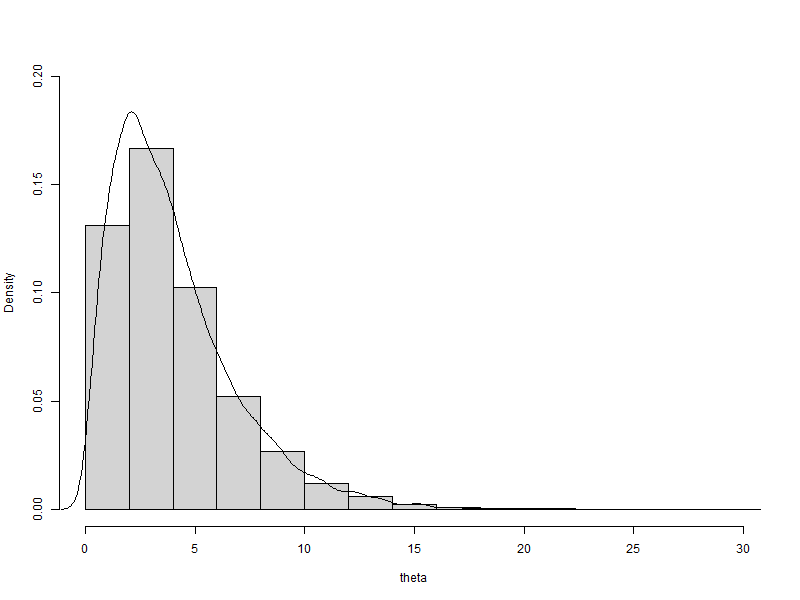
\includegraphics[width =0.6\textwidth]{figure_man/gamdistri_monte_carlo.png}
\end{center}

% \framebreak
%
% Schätzung des Posterior-Erwartungswertes $\hat{E}(\theta | \xv)$

\begin{verbatim}
(Etheta = mean(theta)) # MC estimator
## [1] 4.007281
(se.Etheta = sqrt(var(theta) / T)) # variance
## [1] 0.02841768
shape * 1 / rate # Theoretical expectation
## [1] 4
\end{verbatim}


% \framebreak
%
% Schätzung des Posterior-Verteilungsfunktion $P(\theta > 5) | \xv)$

\begin{verbatim}
(Ptheta = mean(theta > 5)) # MC Estimator
## [1] 0.2863
(se.Ptheta = sqrt(var(theta > 5) / T)) # variance
## [1] 0.004520539
1 - pgamma(5, shape = shape, rate = rate) # theo value
## [1] 0.2872975
f = function(x) {dgamma(x, shape = shape, rate = rate)}
integrate(f, 5, Inf) # Numerical integration in R
## 0.2872975 with absolute error < 9.3e-05
\end{verbatim}

% \framebreak

% \textbf{Highest Posterior Density (HPD)}

% \lz

% HPD Intervalle können ebenfalls konsistent geschätzt werden. HPD Intervalle haben die minimale
% Range von allen möglichen Konfidenzintervallen für ein vorgegebenes $\alpha$, z.B.,
% $\alpha = 0.95$.
% \begin{itemize}
% \item Sortiere $\theta^{(1)} \leq \cdots \leq \theta^{(T)}$.
% \item Empirische Konfidenzintervalle mit $\alpha = 0.95$ und $T = 100$:
%   {\small
%   $$
%   [\theta^{(1)}, \theta^{(95)}], [\theta^{(2)}, \theta^{(96)}], [\theta^{(3)}, \theta^{(97)}],
%     [\theta^{(4)}, \theta^{(98)}], [\theta^{(5)}, \theta^{(99)}], [\theta^{(6)}, \theta^{(100)}].
%   $$
%   }
% \item HPD ist jenes Intervall mit der geringsten Breite.
% \end{itemize}

% \lz

% Der Posterior Modus kann ebenfalls mit Hilfe des HPD-Intervalls und bspw.\ $\alpha = 0.99$
% geschätzt werden. Der Modus ist dann in der Mitte des Intervalls (nicht unbedingt elegant, aber
% auch nicht viel schlechter wie andere Methoden).

% \framebreak

% <<>>=
% hpd = function(x, prob = 0.05) {
%   T = length(x)
%   x = sort(x)
%   gap = max(1, min(T - 1, round(T * (1 - prob))))
%   j = 1:(T - gap)
%   i = which.min(x[j + gap] - x[j])
%   int_hpd = x[c(j[i], j[i] + gap)]
%   int_et = quantile(x, prob = c(prob / 2, 1 - prob / 2))
%   names(int_hpd) = names(int_et) = c(
%     paste(round(prob / 2 * 100, 2), "%", sep = ""),
%     paste(round((1 - prob / 2) * 100, 2), "%", sep = "")
%   )
%   int = rbind("HPD" = int_hpd, "Equi-tailed" = int_et)
%   return(int)
% }
% @

% \framebreak

% <<>>=
% hpd(theta)
% @
% \begin{center}
% <<echo=FALSE>>=
% hist(theta, freq = FALSE, ylim = c(0, 0.2), main = "")
% lines(density(theta))
% int = hpd(theta)
% library("colorspace")
% col = rainbow_hcl(2)
% abline(v = int[1, ], col = col[1], lwd = 2)
% abline(v = int[2, ], col = col[2], lwd = 2)
% legend("topright", c("HPD", "Equi-tailed"), lwd = 2, col = col,
%   box.col = NA, bg = NA)
% @
% \end{center}

% \framebreak

% <<>>=
% int = hpd(theta, prob = 0.99)
% (mode = mean(int["HPD", ])); (shape - 1) * 1 / rate
% @
% \begin{center}
% <<echo=FALSE>>=
% hist(theta, freq = FALSE, ylim = c(0, 0.2), main = "")
% lines(density(theta))
% abline(v = mode, col = col[1], lwd = 2)
% legend("topright", c("mode"), lwd = 2, col = col[1],
%   box.col = NA, bg = NA)
% @
% \end{center}

% \framebreak

% \textbf{Importance Sampling}
%
% Erweiterung von Monte-Carlo, wenn Samples nicht direkt von $f(\theta | \xv)$ erzeugt werden können.
%
% \lz
%
% Wenn Zufallszahlen aus $f^\star(\theta)$ generiert werden können, dann kann der Posterior-Erwartungswert durch
% $$
% E(g(\theta) | \xv) = \int g(\theta) \frac{f(\theta | \xv)}{f^\star(\theta)} f^\star(\theta)d\theta
% $$
% berechnet werden. Die Schätzung basierend auf den Samples aus $f^\star(\theta)$ ist dann
% $$
% \hat{E}(g(\theta) | \xv) = \frac{1}{\sum_{t = 1}^T \omega_t} \sum_{t = 1}^T \omega_t g(\theta^{(t)}),
% $$
% mit $\omega_t = f(\theta^{(t)} | \xv) / f^\star(\theta^{(t)})$.
%
% \framebreak
%
% <<>>=
% T = 10000; shape = 2; rate = 1 / 2
% u = runif(T, 0, 1000)
% w = dgamma(u, shape = shape, rate = rate) / (1 / 1000)
% (Etheta = sum(u * w) / sum(w))
% shape * 1 / rate
% @
%
% \framebreak

% \textbf{Slice Sampling}

% Slice Sampling beruht auf der Eigenschaft, dass Zufallszahlen aus einer Dichtefunktion auch mittels
% gleichverteilter Zufallszahlen die unterhalb von $f(\theta | x)$ liegen erzeugt werden können.

% \lz

% D.h., alle Punkte $(\theta, u)$ für die gilt $0 \leq u \leq f(\theta | x)$.

% \lz

% Algorithmus (stark vereinfacht):
% \begin{itemize}
% \item Initialisiere Startwert $\theta^{(0)}$.
% \item Sample $u \sim U(0, f(\theta^{(t)} | x))$.
% \item Sample $\theta^{(t + 1)} \sim U(s)$ mit $s = \{ \theta^\star : f(\theta^\star | x) \leq u \}$.
% \end{itemize}

% \framebreak

% <<fig.height=3.5, fig.width=5.95>>=
% f = function(x) {
%   dgamma(x, shape = 2, rate = 1 / 2)
% }
% curve(f, 0, 20)
% @
% <<>>=
% find.slice = function(x, fx, f, w = 0.001) {
%   left = right = x
%   repeat {
%     if(f(left) <= fx) break
%     left = left - w
%   }
%   repeat {
%     if(f(right) <= fx) break
%     right = right + w
%   }
%   c(left, right)
% }
% @

% \framebreak

% \begin{center}
% <<>>=
% find.slice(5, 0.08, f)
% @
% <<echo=FALSE, fig.height=3.5, fig.width=5.95>>=
% curve(f, 0, 20)
% slice = find.slice(5, 0.08, f)
% lines(slice, f(slice))
% points(slice, f(slice), pch = 16)
% @
% \end{center}

% \framebreak

% <<>>=
% slicer = function(n, f, w = 0.001, start = 1) {
%   x = start
%   samples = NULL
%   for(i in 1:n) {
%     u = runif(1, 0, f(x))
%     slice = find.slice(x, u, f, w)
%     x = runif(1, slice[1], slice[2])
%     samples = c(samples, x)
%   }
%   return(samples)
% }
% @

% \framebreak

% <<fig.height=3.5, fig.width=5.95>>=
% x = slicer(1000, f, start = 2)
% @
% \begin{center}
% <<echo=FALSE, fig.height=3.5, fig.width=5.95>>=
% hist(x, freq = FALSE, main = "", ylim = c(0, 0.2))
% lines(density(x))
% curve(f, 0, 20, col = "red", add = TRUE)
% @
% \end{center}
\end{vbframe}


\endlecture
\end{document}
